\documentclass[10pt]{standalone}
\usepackage{tikz}
\begin{document}
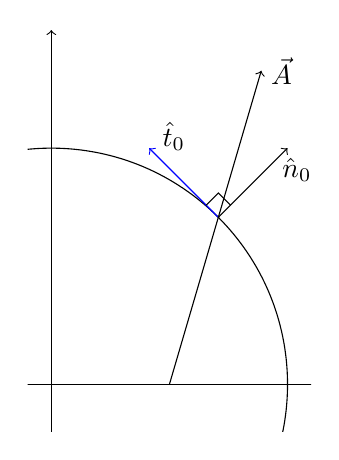
\begin{tikzpicture}[scale=3]
\clip (-0.1,-0.2) rectangle(1.1,1.51);
%\draw[step=.5cm,gray,very thin](-1.4,-1.4) grid(1.4,1.4);
\draw[->](-1.5,0)--(1.5,0);
\draw[->](0,-1.5)--(0,1.5);
\draw(0,0) circle[radius=1cm];
\draw[->](0.7071,0.7071)--(1,1);
\node[below] at (1.04,1){$\hat n_{0}$};
\draw[->,rotate around={90:(0.7071,0.7071)},blue](0.7071,0.7071)--(1,1);
\draw[rotate around={45:(0.7071,0.7071)}] (0.78,0.7071)|-(0.7071,0.78);
\node[right] at (0.43,1.05){$\hat t_{0}$};
\draw[->](0.5,0)--(0.8889,1.3278);
\node[right] at (0.8889,1.3278){$\vec A$};
\end{tikzpicture}
\end{document}